\pgfplotsset{
    every axis/.append style={
        line width=0.8pt,
        tick style={line width=0.8pt, color=black}
    }
}
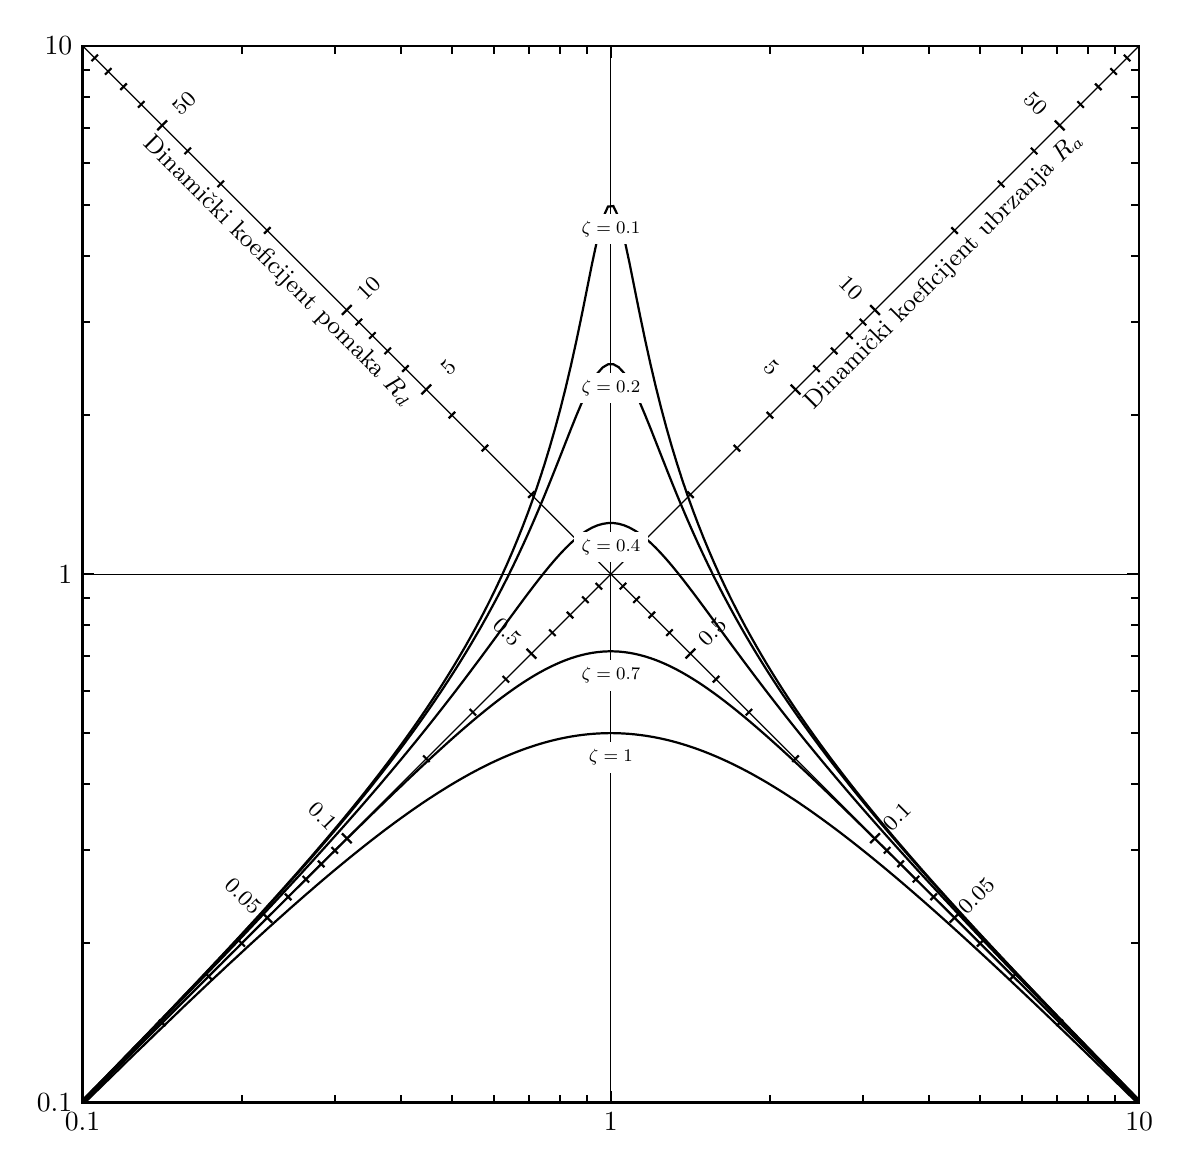
\begin{tikzpicture}%[scale=0.7]
    \begin{loglogaxis} [
        width=15cm,height=15cm,
        xmin = 0.1, xmax = 10.0,
        ymin = 0.1, ymax = 10.0,
        log ticks with fixed point,
        ]
        \pgfplotsinvokeforeach{0.01,0.02,0.03,0.04,0.06,0.07,0.08,0.09,
                               0.2,0.3,0.4,0.6,0.7,0.8,0.9,
                               2,3,4,6,7,8,9,
                               20,30,40,60,70,80,90,100}
        {
            \draw[shift={(#1^0.5,#1^0.5)},rotate=45]
                    (1,1.02)--(1,0.98);

            \draw[shift={(1/#1^0.5,1/#1^-0.5)},rotate=135] 
                    (1,1.02)--(1,0.98);
        }

        \pgfplotsinvokeforeach{0.05,0.1,0.5,5,10,50}
        {
            \draw[shift={(#1^0.5,#1^0.5)},rotate=45]
                    (1,1.03)--(1,0.97);

            \draw[shift={(1/#1^0.5,1/#1^-0.5)},rotate=135] 
                    (1,1.03)--(1,0.97);

            %(sqrt(i)) + sqrt{i} * 0.1; sqrt{i} + sqrt{i}*0.1
            \node[shift={({#1^0.5-(#1^0.5)/10},{#1^0.5+(#1^0.5)/10})},rotate=-45]
                at(1, 1) {\footnotesize{$#1$}};

            %1/(sqrt(i)) + 1/(sqrt{i}) * 0.1; sqrt{i} + sqrt{i}*0.1
            \node[shift={({1/#1^0.5+1/#1^0.5*0.1},{#1^0.5+#1^0.5*0.1})},rotate=45]
                at(1, 1) {\footnotesize{$#1$}};
        }

        \node[rotate=45,anchor=north] at(4,4) {\small{Dinamički koeficijent ubrzanja $R_a$}};
        \node[rotate=-45,anchor=north] at(0.25,4) {\small{Dinamički koeficijent pomaka $R_d$}};
        \draw[thin](1,0.1)--(1,10);
        \draw[thin](0.1,1)--(10,1);
        \draw[thin](0.1,0.1) -- (10,10);
        \draw[thin](10.0,0.1)--(0.1,10);

        %graf
        \foreach \i in {1, 0.7, 0.4, 0.2, 0.1}
        {
            \addplot [
                domain=0.1:10.0,
                samples=200,
            ]
            {x/((1-x^2)^2 + (2*\i*x)^2)^(0.5)};
        }

        \pgfplotsinvokeforeach{1,0.7,0.4, 0.2, 0.1}
        {
            \node[rectangle,fill=white,scale=0.8] at(1,{(1-0.1)/(2*#1)})
            {\footnotesize{$\zeta=#1$}};
        }
%        \draw[thin] (1,5)--(1.5,5);
%        \draw node[rectangle, fill=white, scale=0.8] at(1.5,5){\footnotesize{$\zeta=0.1$}};
    \end{loglogaxis}
\end{tikzpicture}
